\documentclass[a4paper,10pt]{minimal}

\usepackage{tikz}
\usepackage[left=0.5in,right=0.5in,top=1.0in,bottom=1.0in]{geometry}

\begin{document}

\begin{center}
  \textbf{OpenStax Component Overview}
\end{center}

\vspace{1cm}

\begin{tabular}{ p{1.5in} p{5.5in} }
  W\&N         & Words and Numbers team (remote);
                 providers of assessments
                 (aka exercises, questions) \\
  CNX          & archives/serves book content \\
  EXERCISES    & archives/serves assessments \\
  EXCHANGE     & archives/serves ``de-identified'' learners' exercise responses and grades \\
  TUTOR JS     & browser-based, user-facing UI code \\
  TUTOR SERVER & server-based, behind-the-scenes coordinator
                 for Course activities
                 (managing rosters, assignments, content, etc.) \\
  BIGLEARN     & machine-learning (ML) algorithms
                 which understand/predict learners'
                 current level of understanding estimates (CLUEs)
                 and recommend personalized exercises \\
  CC PLUGIN    & Concept Coach javascript plugin
\end{tabular}

\vspace{1cm}

\begin{center}
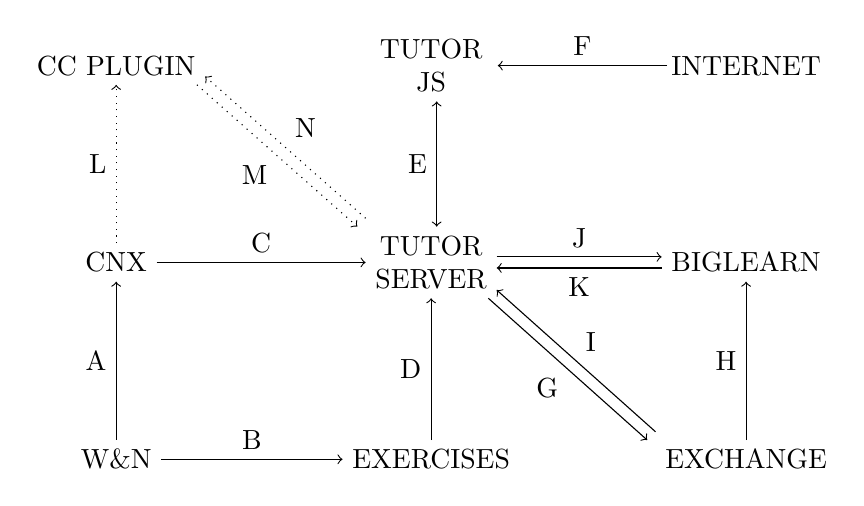
\begin{tikzpicture}
  \node[align=center] (TS)   at (+0.0,+0.0) {TUTOR\\SERVER};
  \node[align=center] (TJS)  at (+0.0,+2.5) {TUTOR\\JS};
  \node[align=center] (CCP)  at (-4.0,+2.5) {CC PLUGIN};
  \node[align=center] (IN)   at (+4.0,+2.5) {INTERNET};
  \node[align=center] (BL)   at (+4.0,+0.0) {BIGLEARN};
  \node[align=center] (CNX)  at (-4.0,+0.0) {CNX};
  \node[align=center] (EXS)  at (+0.0,-2.5) {EXERCISES};
  \node[align=center] (EXC)  at (+4.0,-2.5) {EXCHANGE};
  \node[align=center] (WN)   at (-4.0,-2.5) {W\&N};

  \path[->,transform canvas={xshift=+0.0em}] (WN)  edge node[left]  {A} (CNX);
  \path[->,transform canvas={yshift=+0.0em}] (WN)  edge node[above] {B} (EXS);

  \path[->,transform canvas={yshift=+0.0em}] (CNX) edge node[above] {C} (TS);
  % \path[->,transform canvas={yshift=+0.2em}] (TS)  edge node[above] {K} (CNX);

  \path[->,transform canvas={xshift=+0.0em}] (EXS) edge node[left] {D} (TS);
  % \path[->,transform canvas={xshift=-0.2em}] (TS)  edge node[left]  {E} (EXS);

  \path[<->,transform canvas={xshift=+0.2em}] (TS)  edge node[left]  {E} (TJS);

  \path[->,transform canvas={xshift=+0.2em}] (IN)  edge node[above] {F} (TJS);

  \path[->,transform canvas={xshift=-0.3em}] (TS.south east)  edge node[below left]  {G} (EXC.north west);
  \path[->,transform canvas={yshift=+0.3em}] (EXC.north west) edge node[above right] {I} (TS.south east);

  \path[->,transform canvas={xshift=+0.0em}] (EXC) edge node[left] {H} (BL);

  \path[->,transform canvas={yshift=+0.2em}] (TS) edge node[above] {J} (BL);
  \path[->,transform canvas={yshift=-0.2em}] (BL) edge node[below] {K} (TS);

  \path[->,dotted,transform canvas={xshift=+0.0em}] (CNX)  edge node[left]  {L} (CCP);

  \path[->,dotted,transform canvas={xshift=-0.3em}] (CCP.south east) edge node[below left]  {M} (TS.north west);
  \path[->,dotted,transform canvas={yshift=+0.3em}] (TS.north west)  edge node[above right] {N} (CCP.south east);

\end{tikzpicture}
\end{center}

\vspace{1cm}

\begin{tabular}{ p{0.5in} p{6.5in} }
  A & W\&N provides content-based assessments to CNX \\
  B & W\&N provides exercises and exercise-tag spreadsheets
      for import into EXERCISES \\
  C & TUTOR SERVER pulls/processes book content from CNX \\
  D & TUTOR SERVER pulls/processes assessments from EXERCISES \\
  E & TUTOR SERVER and TUTOR JS exchange information based on user's actions \\
  F & TUTOR JS pulls some content (images, videos, etc.)
      from internet sites (Khan Academy, etc.)
      as directed by TUTOR SERVER's processed content \\
  G & TUTOR SERVER (a) requests learner ``de-identifiers'' from EXCHANGE and
                   (b) sends ``de-identified'' learner responses and grades to EXCHANGE
                       as learners complete assessments in homeworks, readings, etc. \\
  H & EXCHANGE sends BIGLEARN learner ``de-identifiers''
      and ``de-identified'' learner responses and grades \\
  I & EXCHANGE returns learner ``de-identifiers'' to TUTOR SERVER \\
  J & TUTOR SERVER sends (a) assessment ids and tags and
                         (b) assessment pool information
      to BIGLEARN and requests (a) personalized exercises and
                               (b) learner CLUEs
      from BIGLEARN \\
  K & BIGLEARN returns (a) assessment pool identifiers,
                       (b) personalized assessment selections and
                       (c) learner CLUEs
      to TUTOR SERVER \\
  L & CNX places CC PLUGIN in CC-enabled pages \\
  M & CC PLUGIN (a) requests assessments from TUTOR SERVER and
                (b) sends learner responses to TUTOR SERVER \\
  N & TUTOR SERVER sends assessments to CC PLUGIN
\end{tabular}

\end{document}

